
\item A glass capillary tube is of the shape of a truncated cone with an apex angle \emph{also} that its two ends have cross sections of different radii. When dipped in water vertically, water rises in it to a height \( h \), where the radius of its cross section is \( b \). If the surface tension of water is \( S \), its density is \( \rho \), and its contact angle with glass is \( \theta \), the value of \( h \) will be (\( g \) is the acceleration due to gravity)
    \begin{center}
        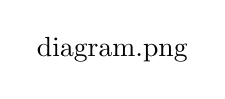
\begin{tikzpicture}
            \node at (0, 0) {diagram.png};
        \end{tikzpicture}
    \end{center}
    \begin{tasks}(2)
        \task \(\frac{2S}{b\rho g}\cos(\theta - \alpha)\)
        \task \(\frac{2S}{b\rho g}\cos(\theta + \alpha)\)
        \task \(\frac{2S}{b\rho g}\cos(\theta - \frac{\alpha}{2})\)
        \task \(\frac{2S}{b\rho g}\cos(\theta + \frac{\alpha}{2})\)
    \end{tasks}
